\documentclass[a4paper,twocolumn]{article}
\author{José Duarte}
\title{Concurrency \& Parallelism\\Test 2 - 2015/16}
\usepackage{geometry}
\geometry{
    top=15mm,
    right=10mm,
    left=10mm,
    heightrounded
}
\usepackage{listings}
\lstset{basicstyle=\ttfamily}
\usepackage{amsmath}
\usepackage{graphicx}
\usepackage{hyperref}
\begin{document}
\maketitle
\section{Question 1}
\paragraph{Competition}
Accessing a critical section, threads have to compete to get time over the critical section.
\paragraph{Cooperation}
A barrier is useful to make processes wait on each other,
e.g. we have function $f(x, y)$ and both $x$ and $y$ are results from other functions running concurrently,
to run $f$ we need to wait on both.
\section{Question 2}
\subsection{a)}
\begin{tabular}{c|c}
    Smallest & 11 \\
    \hline
    Largest  & 11 \\
\end{tabular}
\subsection{b)}
\begin{tabular}{c|c c c}
    Smallest & 11 & 11 & 11 \\
    \hline
    Largest  & 11 & 11 & 11 \\
\end{tabular}
\subsection{c)}
\begin{tabular}{c|c c c}
    Smallest & 3 & 4 & 5 \\
    \hline
    Largest  & 9 & 10 & 11\\
\end{tabular}
\section{Question 3}
\begin{tabular}{c | l}
    $x$ & $ 2, 4, 5, 6$ \\
    \hline
    $y$ & $1, 3, 4$ \\
    \hline
    $(x, y)$ & $(2, 1), (4, 3), (4, 4), (5, 3), (5, 4), (6, 4)$ \\
\end{tabular}

\section{Question 4}
\section{Question 5}
\begin{itemize}
    \item F
    \item T
    \item F
    \item F
    \item F
    \item F
    \item T
    \item F
    \item F
    \item T
    \item F
    \item T
    \item F
    \item F
    \item T
    \item T
\end{itemize}
\section{Question 6}
\begin{itemize}
    \item Deadlock - Progress
    \item Livelock - Progress
    \item Starvation - Progress
    \item Busy-Waiting - Progress
    \item All threads simultaneously execute a \texttt{lock(X)} over the same lock variable X - Progress
    \item All threads simultaneously execute a \texttt{compareAndSwap(X,v)} over the same variable X - No Progress
\end{itemize}
\section{Question 7}
\subsection{a)}
See \autoref{q7:a}
\begin{figure}[h]
    \centering
    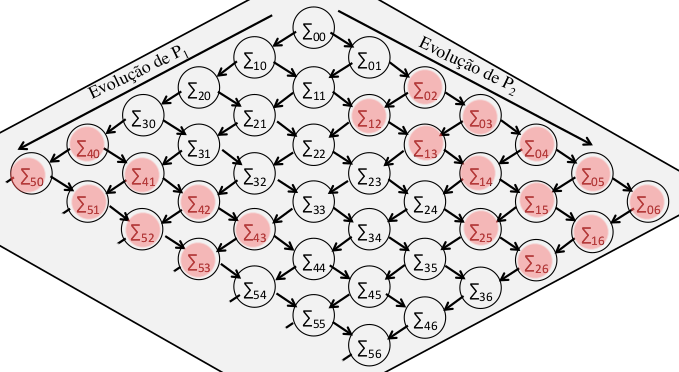
\includegraphics[width=0.9\linewidth]{q7a.png}
    \caption{}
    \label{q7:a}
\end{figure}
\subsection{b)}
\subsubsection{i)}
$$
\Sigma_{00}, \Sigma_{10}, \Sigma_{20}, \Sigma_{30},
\Sigma_{31}, \Sigma_{32}, \Sigma_{33}, \Sigma_{34},
\Sigma_{44}, \Sigma_{54}, \Sigma_{55}, \Sigma_{56}
$$
\subsubsection{ii)}
$$
\Sigma_{00}, \Sigma_{01}, \Sigma_{02}, \Sigma_{03},
\Sigma_{31}, \Sigma_{32}, \Sigma_{33}, \Sigma_{34},
\Sigma_{44}, \Sigma_{54}, \Sigma_{55}, \Sigma_{56}
$$
\subsubsection{iii)}
\subsubsection{iv)}
\subsubsection{v)}

\section{Question 8}
\begin{lstlisting}
Node oldTop = top.get();
node.next = oldTop;
return = top.compareAndSet(oldTop, node);
\end{lstlisting}
\section{Question 9}
\end{document}